\begin{figure}[!h]
\centering
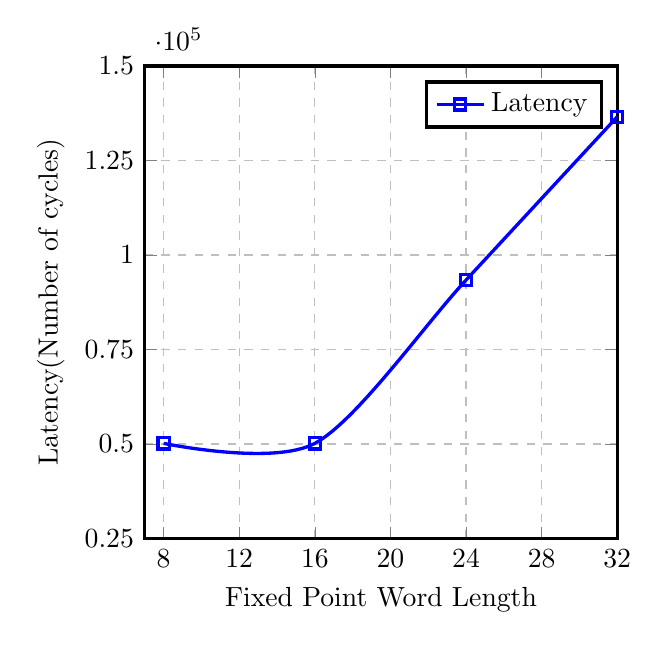
\begin{tikzpicture}
\begin{axis}[
scale only axis,
height=6cm,
width=6cm,
    xlabel={Fixed Point Word Length},
    ylabel={Latency(Number of cycles)},
    xmin=7, xmax=32,
    ymin=25000, ymax=150000,
    xtick={8,12,16,20,24,28,32},
    ytick={25000,50000,75000,100000,125000,150000},
    legend pos=north east,
    ymajorgrids=true,
    xmajorgrids=true,
    grid style=dashed,
    very thick
]
\addplot[
    color=blue,
    mark=square,
    smooth
    ]
    coordinates {
    (32,136562)(24,93362)(16,50162)(8,50162)
    };
    \addlegendentry{Latency}
\end{axis}
\end{tikzpicture}
\caption{Effect of varying the Fixed Point Word Length on Latency}
\label{fig:5.6}
\end{figure}